\documentclass[tikz, border=14pt]{standalone}
\usepackage{tikz}
\usetikzlibrary{positioning, fit, calc, shapes.geometric, shapes.symbols, arrows.meta, backgrounds}

%% ── Palette ────────────────────────────────────────────────────────────────
\definecolor{clBlue}    {RGB}{219,234,254}  % submission fill
\definecolor{clBlueBd}  {RGB}{ 59,130,246}  % submission border
\definecolor{clOrange}  {RGB}{255,237,213}  % worker fill
\definecolor{clOrangeBd}{RGB}{234, 88, 12}  % worker border
\definecolor{clGreen}   {RGB}{220,252,231}  % outbox fill
\definecolor{clGreenBd} {RGB}{ 22,163, 74}  % outbox border
\definecolor{clRed}     {RGB}{254,226,226}  % proddb fill
\definecolor{clRedBd}   {RGB}{220, 38, 38}  % proddb border
\definecolor{clPurple}  {RGB}{237,233,254}  % container bg
\definecolor{clPurpleBd}{RGB}{109, 40,217}  % container border
\definecolor{clArrow}   {RGB}{107,114,128}  % arrows

%% ── Global node styles ────────────────────────────────────────────────────
\tikzset{
  %% rounded process box
  proc/.style={
    rectangle, rounded corners=6pt,
    minimum width=3.2cm, minimum height=1.1cm,
    align=center, font=\small\sffamily,
    inner sep=8pt, draw, thick
  },
  %% cylinder (database)
  db/.style={
    cylinder, shape border rotate=90, aspect=0.22,
    minimum width=3.2cm, minimum height=1.3cm,
    align=center, font=\small\sffamily,
    inner sep=6pt, draw, thick
  },
  %% colour variants
  blue/.style   ={proc, fill=clBlue,   draw=clBlueBd,   text=clBlueBd},
  orange/.style ={proc, fill=clOrange, draw=clOrangeBd, text=clOrangeBd},
  green/.style  ={db,   fill=clGreen,  draw=clGreenBd,  text=clGreenBd},
  red/.style    ={db,   fill=clRed,    draw=clRedBd,    text=clRedBd},
  %% arrows
  arr/.style={
    -{Stealth[length=7pt, width=5pt]},
    thick, color=clArrow
  },
  arrDash/.style={arr, dashed},
  lbl/.style={
    font=\scriptsize\sffamily, text=clArrow,
    fill=white, inner sep=2pt, rounded corners=2pt
  }
}

\begin{document}
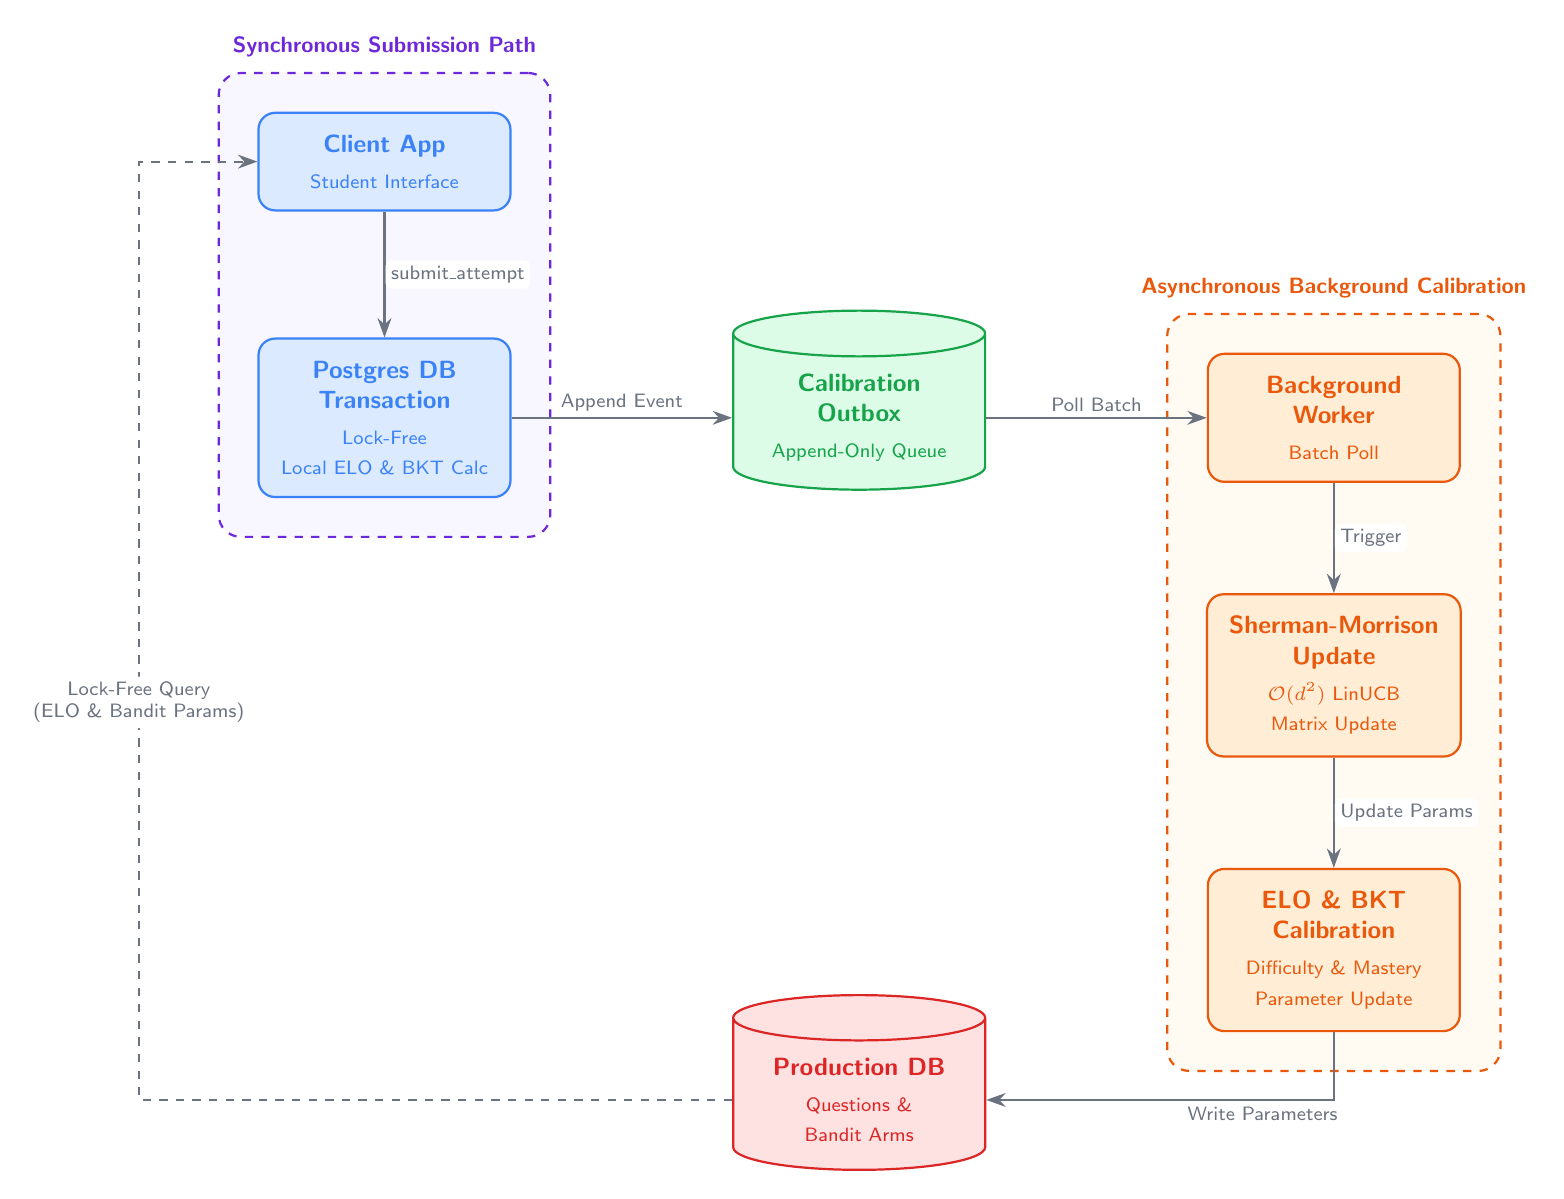
\begin{tikzpicture}[node distance=1.2cm and 2.6cm]

%% ═══════════════════════════════════════════════════════════════
%%  COLUMN 1 — Synchronous Submission Path
%% ═══════════════════════════════════════════════════════════════

\node[blue] (client) {
  \textbf{Client App}\\[2pt]
  \scriptsize Student Interface
};

\node[blue, below=1.6cm of client] (txn) {
  \textbf{Postgres DB}\\
  \textbf{Transaction}\\[2pt]
  \scriptsize Lock-Free\\
  \scriptsize Local ELO \& BKT Calc
};

%% container box — Synchronous Path
\begin{scope}[on background layer]
  \node[
    rectangle, rounded corners=8pt,
    fill=clPurple!40, draw=clPurpleBd, dashed, thick,
    fit=(client)(txn), inner sep=14pt
  ] (syncBox) {};
\end{scope}
\node[
  font=\footnotesize\sffamily\bfseries, text=clPurpleBd,
  above=2pt of syncBox.north
] {Synchronous Submission Path};

%% ═══════════════════════════════════════════════════════════════
%%  COLUMN 2 — Calibration Outbox (centre)
%% ═══════════════════════════════════════════════════════════════

\node[green, right=2.8cm of txn] (outbox) {
  \textbf{Calibration}\\
  \textbf{Outbox}\\[2pt]
  \scriptsize Append-Only Queue
};

%% ═══════════════════════════════════════════════════════════════
%%  COLUMN 3 — Asynchronous Background Calibration
%% ═══════════════════════════════════════════════════════════════

\node[orange, right=2.8cm of outbox] (worker) {
  \textbf{Background}\\
  \textbf{Worker}\\[2pt]
  \scriptsize Batch Poll
};

\node[orange, below=1.4cm of worker] (sm) {
  \textbf{Sherman-Morrison}\\
  \textbf{Update}\\[2pt]
  \scriptsize $\mathcal{O}(d^2)$ LinUCB\\
  \scriptsize Matrix Update
};

\node[orange, below=1.4cm of sm] (bkt) {
  \textbf{ELO \& BKT}\\
  \textbf{Calibration}\\[2pt]
  \scriptsize Difficulty \& Mastery\\
  \scriptsize Parameter Update
};

%% container box — Async Background
\begin{scope}[on background layer]
  \node[
    rectangle, rounded corners=8pt,
    fill=clOrange!30, draw=clOrangeBd, dashed, thick,
    fit=(worker)(sm)(bkt), inner sep=14pt
  ] (asyncBox) {};
\end{scope}
\node[
  font=\footnotesize\sffamily\bfseries, text=clOrangeBd,
  above=2pt of asyncBox.north
] {Asynchronous Background Calibration};

%% ═══════════════════════════════════════════════════════════════
%%  PRODUCTION DB — bottom centre
%% ═══════════════════════════════════════════════════════════════

%% Anchor it horizontally between syncBox and asyncBox, below everything
\node[red,
  below=2.4cm of $(syncBox.south)!0.5!(asyncBox.south)$
] (proddb) {
  \textbf{Production DB}\\[2pt]
  \scriptsize Questions \&\\
  \scriptsize Bandit Arms
};

%% ═══════════════════════════════════════════════════════════════
%%  ARROWS — Synchronous Path
%% ═══════════════════════════════════════════════════════════════

\draw[arr] (client) --
  node[lbl, right]{submit\_attempt} (txn);

\draw[arr] (txn.east) --
  node[lbl, above]{Append Event} (outbox.west);

%% ═══════════════════════════════════════════════════════════════
%%  ARROWS — Background Path
%% ═══════════════════════════════════════════════════════════════

\draw[arr] (outbox.east) --
  node[lbl, above]{Poll Batch} (worker.west);

\draw[arr] (worker) --
  node[lbl, right]{Trigger} (sm);

\draw[arr] (sm) --
  node[lbl, right]{Update Params} (bkt);

%% ═══════════════════════════════════════════════════════════════
%%  ARROWS — Write-back to Production DB
%% ═══════════════════════════════════════════════════════════════

%% bkt  →  proddb  (orthogonal: down then left)
\draw[arr] (bkt.south) |-
  node[lbl, below right, pos=0.72]{Write Parameters} (proddb.east);

%% ═══════════════════════════════════════════════════════════════
%%  FEEDBACK LOOP — Production DB → Client App
%% ═══════════════════════════════════════════════════════════════

%% proddb → left → up → client  (orthogonal routing around the left side of syncBox)
\draw[arrDash] (proddb.west) -- 
  ($(syncBox.west|-proddb.west) - (1.0, 0)$) -- 
  node[lbl, align=center, pos=0.5]{Lock-Free Query\\(ELO \& Bandit Params)} 
  ($(syncBox.west) - (1.0, 0)$) |- (client.west);

\end{tikzpicture}
\end{document}
